% -*- root: ../paper.tex -*-


The core component of \systemname is a knowledge-base that is used to identify column names.
The knowledge-base is broken down into two parts, one heuristic-based, and the other feedback-based.
The latter part is used to preserve column names explicitly labeled by the user for future use.  
This is simply a mapping from a table identifier and column position to an explicit name.  
Hence, for the balance of the paper we will focus on the former, more complex heuristic-based part of the \systemname knowledge-base.
Specifically, in this section we define the representational semantics of the heuristic knowledge-base and define the evaluation semantics for labeling and discovery queries.

%%%%%%%%%%%%%%%%%%%%%%%%%%%%%%%%%%%%%%%%%%%%%%%%%%%%%%%%%%%%%%%%%%

\begin{figure}
\centering
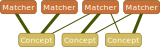
\includegraphics[width=0.8\columnwidth]{graphics/knowledgebase}
\caption{An example \systemname heuristic knowledge-base}
\label{fig:bipartitekb}
\trimfigurespacing
\end{figure}

\subsection{Matchers and Concepts}

The heuristic content of the knowledge base is best expressed as a bipartite graph between \emph{matchers} and \emph{concepts}.
An example is shown in Figure~\ref{fig:bipartitekb}.  
A matcher is any function $M : T[A] \rightarrow [0,1]$ which assigns any column of data to a $[0,1]$-valued measure that we call the matcher's \emph{score} for the column.  
Concepts correspond to names.
However, because the same name may be used in different contexts, multiple concepts can use the same column name.
Similarly, a single concept may be identified by multiple synonymous names, so a single concept may be associated with multiple names.
An edge between a matcher and a concept indicates candidacy:
For a given column ranked highly by a matcher, any concept linked to the matcher by an edge is a viable name for the column.
Each matcher has a \emph{default} edge, indicated in Figure~\ref{fig:bipartitekb} in bold.

Formally, a knowledge-base $\textbf{KB} = \tuple{\mathbb M, \mathbb C, \mathbb E}$, with matchers $M \in \mathbb M$, concepts $C \in \mathbb C$, edge matrix $\mathbb E : \mathbb M \times \mathbb C \rightarrow \{\mathbf D, \top, \bot\}$.
Specifically $\mathbb E(M, C) \in \{\mathbf D, \top\}$ indicates an edge between $M$ and $C$.
The value $\mathbf D$ identifies the default edge.
We require that each matcher have exactly one default edge.
$$\forall M \in \mathbb M \;\;\; \exists C \in \mathbb C\;\;\; \mathbb E(M, C) = \mathbf D$$
$$\forall M \in \mathbb M, C_1 \in \mathbb C \;\;\; \not\exists C_2 \neq C_1 \in \mathbb C \;\;\; \mathbb E(M, C_1) = \mathbb E(M, C_2) = \mathbf D$$
We denote by $\mathbb D(M)$ the concept connected to $M$ by default edge, and by $\textbf{name}(C)$ the set of (synonymous) names associated with a concept.



%%%%%%%%%%%%%%%%%%%%%%%%%%%%%%%%%%%%%%%%%%%%%%%%%%%%%%%%%%%%%%%%%%

\subsection{Query Semantics}

The \systemname knowledge-base is responsible for answering both labeling and discovery queries.
For this paper, we adopt a simplified model where the answers to both types of queries depend solely on the highest score assigned to a column by a relevant matcher.
This simplification carries two immediate limitations.
First, query answering semantics do not attempt to combine inputs from multiple matchers --- only the matcher with the highest score is used.
However, we do discuss in Section~\ref{sec:expertui} how expert feedback can be used to derive new matchers from existing ones.
Second, this simplification precludes the use of contextual information about the table.
For example, features like ``the table describes medical data'' could be used to significantly improve result quality.
Although we do not address the use of context in this paper, we outline some potential approaches while discussing future work in Section~\ref{sec:future}.

\tinysection{Labeling}
The input to a labeling query is a set of columns $T_C = \{A_1, \ldots, A_N\}$ and the knowledge-base $\tuple{\mathbb M, \mathbb C, \mathbb E}$. 
The goal of the query is to identify a list of $N$ \emph{distinct} concepts $C_1, \ldots, C_N$, one for each attribute, that best fit data in the columns.
This can be phrased as a simple linear optimization problem that identifies $N$ matchers $M_1, \ldots, M_N$ that maximize the sum:
\begin{align*}
\sum_{i \in [1,N]} M_i(A_i) 
&\;\;\;\;\; \textbf{subject to} &
\forall i \neq j \;\;\; D(M_i) \neq D(M_j)
\end{align*}
The concepts in the result are given by the resulting matcher's default edges $C_i = D(M_i)$.

\tinysection{Discovery}
The input to a labeling query is a name $\nu$, a set of columns $T_C = \{A_1, \ldots, A_N\}$, and the knowledge-base $\tuple{\mathbb M, \mathbb C, \mathbb E}$. 
The goal of the query is to identify the position of the attribute $i \in [0,N]$ most likely to fit the column name.
The set of matchers that can be used to identify this column are given by:
$$\textbf{candidates}_\nu = \comprehension{M}{E(M, C) \neq \bot \wedge \nu \in \textbf{name}(C)}$$
The answer to the discovery query then is given by
$$\argmax_{i \in [0,N]} \left( \max_{M \in \textbf{candidates}_\nu} M(A_i)\right)$$

\subsection{Constructing a Knowledge Base}
To instantiate specific match-quality functions, we merge three sources of information: Learned Heuristics, Expert Augmentations, and User Feedback. 
The first category, learned heuristics, models the content and distribution of typical instances of columns with a similar name.
This distribution serves as a baseline match-quality function.
The second category, expert augmentations, modifies the first, increasing or decreasing values based on expert-provided descriptions of what should and should not appear in columns with this name.
The final category, user feedback, provides users with a way to confirm or override automated system choices, while also preserving these associations for future use.

